%%%%%%%%%%%%%%%%%%%%%%%%%%%%%%%%%%%%%%%%%%%%%%
% An example of a lab report write-up.
%%%%%%%%%%%%%%%%%%%%%%%%%%%%%%%%%%%%%%%%%%%%%%
% This is a combination of several labs that I have done in the past for
% Computer Engineering, so it is not to be taken literally, but instead used as
% a great starting template for your own lab write up.  When creating this
% template, I tried to keep in mind all of the functions and functionality of
% LaTeX that I spent a lot of time researching and using in my lab reports and
% include them here so that it is fairly easy for students first learning LaTeX
% to jump on in and get immediate results.  However, I do assume that the
% person using this guide has already created at least a "Hello World" PDF
% document using LaTeX (which means it's installed and ready to go).
%
% My preference for developing in LaTeX is to use the LaTeX Plugin for gedit in
% Linux.  There are others for Mac and Windows as well (particularly MikTeX).
% Another excellent plugin is the Calc2LaTeX plugin for the OpenOffice suite.
% It makes it very easy to create a large table very quickly.
%
% Professors have different tastes for how they want the lab write-ups done, so
% check with the section layout for your class and create a template file for
% each class (my recommendation).
%
% Also, there is a list of common commands at the bottom of this document.  Use
% these as a quick reference.  If you'd like more, you can view the "LaTeX Cheat
% Sheet.pdf" included with this template material.
%
% (c) 2009 Derek R. Hildreth <derek@derekhildreth.com> http://www.derekhildreth.com
% This work is licensed under the Creative Commons Attribution-NonCommercial-ShareAlike License. To view a copy of this license, visit http://creativecommons.org/licenses/by-nc-sa/1.0/ or send a letter to Creative Commons, 559 Nathan Abbott Way, Stanford, California 94305, USA.
%%%%%%%%%%%%%%%%%%%%%%%%%%%%%%%%%%%%%%%%%%%%%%


\documentclass[aps,letterpaper,10pt]{revtex4}

\usepackage{graphicx} % For images
\usepackage{float}    % For tables and other floats
\usepackage{verbatim} % For comments and other
\usepackage{amsmath}  % For math
\usepackage{amssymb}  % For more math
\usepackage{fullpage} % Set margins and place page numbers at bottom center
\usepackage{listings} % For source code
\usepackage{subfig}   % For subfigures
\usepackage[utf8]{inputenc}
\usepackage{ctex}	
\usepackage{graphicx}
\usepackage[usenames,dvipsnames]{color} % For colors and names

\definecolor{mygrey}{gray}{.96} % Light Grey
\lstset{
	language=[ISO]C++,              % choose the language of the code ("language=Verilog" is popular as well)
   tabsize=3,							  % sets the size of the tabs in spaces (1 Tab is replaced with 3 spaces)
	basicstyle=\tiny,               % the size of the fonts that are used for the code
	numbers=left,                   % where to put the line-numbers
	numberstyle=\tiny,              % the size of the fonts that are used for the line-numbers
	stepnumber=1,                   % the step between two line-numbers. If it's 1 each line will be numbered
	numbersep=5pt,                  % how far the line-numbers are from the code
	backgroundcolor=\color{mygrey}, % choose the background color. You must add \usepackage{color}
	%showspaces=false,              % show spaces adding particular underscores
	%showstringspaces=false,        % underline spaces within strings
	%showtabs=false,                % show tabs within strings adding particular underscores
	frame=single,	                 % adds a frame around the code
	tabsize=3,	                    % sets default tabsize to 2 spaces
	captionpos=b,                   % sets the caption-position to bottom
	breaklines=true,                % sets automatic line breaking
	breakatwhitespace=false,        % sets if automatic breaks should only happen at whitespace
	%escapeinside={\%*}{*)},        % if you want to add a comment within your code
	commentstyle=\color{BrickRed}   % sets the comment style
}

% Make units a little nicer looking and faster to type
\newcommand{\Hz}{\textsl{Hz}}
\newcommand{\KHz}{\textsl{KHz}}
\newcommand{\MHz}{\textsl{MHz}}
\newcommand{\GHz}{\textsl{GHz}}
\newcommand{\ns}{\textsl{ns}}
\newcommand{\ms}{\textsl{ms}}
\newcommand{\s}{\textsl{s}}



% TITLE PAGE CONTENT %%%%%%%%%%%%%%%%%%%%%%%%
% Remember to fill this section out for each
% lab write-up.
%%%%%%%%%%%%%%%%%%%%%%%%%%%%%%%%%%%%%%%%%%%%%
\newcommand{\labno}{05}
\newcommand{\labtitle}{AI 3603 Artificial Intelligence: Principles and Techniques}
\newcommand{\authorname}{陈路轩 (523030910014)}
\newcommand{\hw}{1}
% END TITLE PAGE CONTENT %%%%%%%%%%%%%%%%%%%%
\renewcommand{\figurename}{Figure}

\begin{document}  % START THE DOCUMENT!


% TITLE PAGE %%%%%%%%%%%%%%%%%%%%%%%%%%%%%%%%%%%%%%
% If you'd like to change the content of this,
% do it in the "TITLE PAGE CONTENT" directly above
% this message
%%%%%%%%%%%%%%%%%%%%%%%%%%%%%%%%%%%%%%%%%%%%%%%%%%%
\begin{titlepage}
\begin{center}
{\Large \textsc{\labtitle} \\ \vspace{4pt}}
\rule[13pt]{\textwidth}{1pt} \\ \vspace{150pt}
{\large By: \authorname \\ \vspace{10pt}
HW\#: \hw \\ \vspace{10pt}
\today}
\end{center}
\end{titlepage}
% END TITLE PAGE %%%%%%%%%%%%%%%%%%%%%%%%%%%%%%%%%%





%%%%%%%%%%%%%%%%%%%%%%%%%%%%%%
%%%%%%%%%%%%%%%%%%%%%%%%%%%%%%
\section{Introduction}
%No Text Here
%%%%%%%%%%%%%%%%%%%%%%%%%%%%%%%
\subsection{Problem background}
Path planning is a fundamental and core problem in the fields of Artificial Intelligence and Robotics. It is crucial for the navigation capabilities of various autonomous systems, such as service robots and self-driving cars. An effective path planning algorithm enables a robot to autonomously navigate from a starting point to a destination in complex environments while avoiding collisions with obstacles.

This assignment focuses on a path-planning framework for a service robot operating in an indoor environment.The specific scenario involves a known 2D global map where the robot must autonomously plan an optimal or near-optimal, collision-free path based on a given start position $(x_s, y_s)$ and goal position $(x_g, y_g)$. To achieve this objective, this assignment will utilize the basic and improved $A^*$ search algorithm as the core technology. The solution will be developed through a series of progressive tasks, starting from implementing basic pathfinding, advancing to enhancing path quality, and culminating in generating a smooth trajectory.


%%%%%%%%%%%%%%%%%%%%%%%%%%%%%%
\subsection{Task Objectives}
This assignment has three core tasks, designed to progressively build a comprehensive path-planning system:
\begin{itemize}
    \item \textbf{Task 1}: To implement the basic A$^*$ algorithm. In this task, the robot is restricted to moving forward, backward, left, and right on a grid map to accomplish fundamental point-to-point pathfinding.

    \item \textbf{Task 2}: To improve the basic A$^*$ algorithm to improve path quality. The requirements involve three aspects: enabling diagonal movement ; considering the distance to obstacles to avoid collisions ; and adding a steering cost to reduce unnecessary turns.

    \item \textbf{Task 3}: To implement a path smoothing algorithm. As the paths generated by the first two tasks are discrete, this task requires transforming the path into a smooth trajectory.
\end{itemize}



%%%%%%%%%%%%%%%%%%%%%%%%%%%%%%
%%%%%%%%%%%%%%%%%%%%%%%%%%%%%%
\newpage
\section{Algorithm Design and Implementation}
\subsection{Task 1: Basic A$^*$ Algorithm}
\subsubsection{Description}
The A$^*$ algorithm is a widely used heuristic search algorithm, renowned for its efficiency and completeness in finding the shortest path. The algorithm evaluates the cost of each node $n$ on a path using an evaluation function, $f(n)$, to determine which node to explore next. In this task, we implement the basic A$^*$ algorithm on a 120m $\times$ 120m grid map, and the robot is restricted to moving only forward, backward, left, and right.

\subsubsection{Formulation}
The core of the A$^*$ algorithm lies in its evaluation function: $f(n) = g(n) + h(n)$.
\begin{description}
	\item[$g(n)$ (Actual Cost)] 
	This value represents the accumulated cost from the starting node to the current node $n$ along the specific path discovered by the algorithm. For this task, since movement is restricted to four directions on a 1.0m $\times$ 1.0m grid, the cost for each step is uniformly 1. Therefore, the formula simplifies to:
	$$g(n) = g(\text{parent}(n)) + 1$$
    \item[$h(n)$ (Heuristic Function)] This value represents the estimated cost from the current node $n$ to the goal node. For a grid map with only four-directional movement, the \textbf{Manhattan Distance} is a highly effective and admissible heuristic function, as it never overestimates the true remaining cost. Its formula is:
    $$h(n) = |x_n - x_g| + |y_n - y_g|$$
    where $(x_n, y_n)$ are the coordinates of the current node and $(x_g, y_g)$ are the coordinates of the goal node.
\end{description}


\subsubsection{Implementation}

\paragraph{Core Data Structures:}
	\begin{enumerate}
		\item \textbf{Node Class}: A Node class is defined. Each instance stores its \texttt{position}, a \texttt{parent\_node} pointer (for path reconstruction), and the three cost values: $g(n)$, $h(n)$, and $f(n)$(total cost).

		\item \textbf{Nodes List}: A list named \texttt{nodes} is implemented as a min-heap using Python's heapq module. This ensures that we can efficiently pop the node with the minimum \texttt{total\_cost} in $O(\log N)$ time complexity.

		\item \textbf{Explored Set}: A variable named \texttt{explored} is implemented as a set, which records which nodes have already been explored , to  avoid redundant computations.
	\end{enumerate}

\paragraph{Algorithm Execution Flow}

\begin{enumerate}
	\item \textbf{Initialization}: Create Start node and Goal node, then push the start node into the min-heap to begin the search.

	\item \textbf{Main Loop}: As long as the \texttt{nodes} heap is not empty, pop the node with the lowest \texttt{total\_cost}, from the heap.

	\item \textbf{Goal Test}:Check the popped node to see if it is the goal. If so, the path is reconstructed by backtracking from the goal node via the \texttt{parent\_node} pointers, then reverse it. If not, proceed to expand its neighbors.

	\item \textbf{Neighbor Expansion}: For the current node, its four neighbors (forward, backward, left, right) are generated.

	\item \textbf{Validation}: Before processing each neighbor, a three-fold check is performed to ensure it is: within the map boundaries, not an obstacle, and not already in the \texttt{explored} set. Discard the invalid ones.

	\item \textbf{Cost Calculation}: Calculate each valid neighbor's $g(n)$, $h(n)$, and $f(n)$ values . Then push it into the min-heap .
\end{enumerate}

\subsubsection{Result}
\begin{figure}[h!]
    \centering % 图片居中显示
    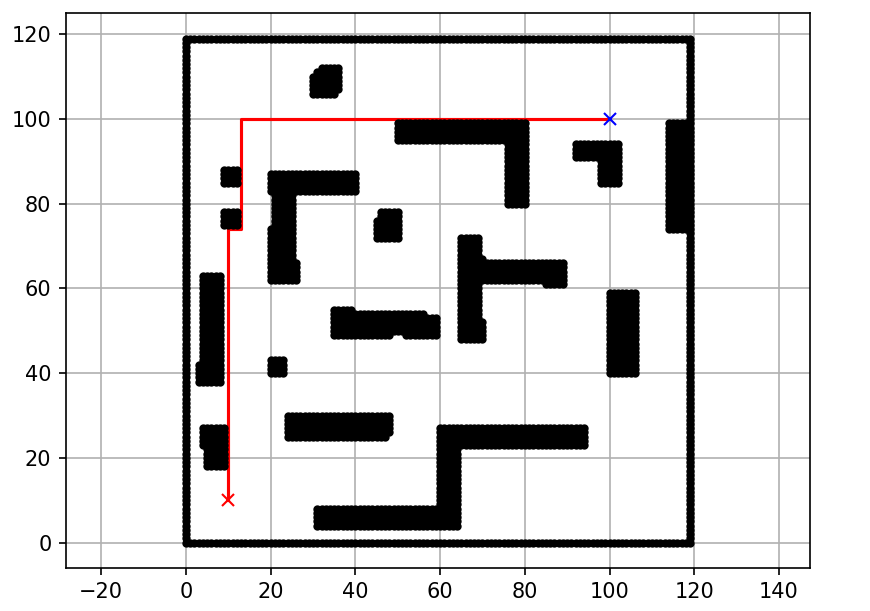
\includegraphics[width=0.4\textwidth]{task1.png} % 插入图片,设置宽度为文本宽度的一半
    \caption{Path for task1} % 设置图片标题
    \label{fig:logo} % 设置标签,用于在文本中引用
\end{figure}
As shown in the figure , our algorithm has effectively planned a valid, collision-free path from the start position (red 'x') to the goal position (blue 'x') on the given grid map.

\newpage
\subsection{Task 2: Improved A$^*$ Algorithm}
\subsubsection{Description}
In Task 2, we implement an improved A$^*$ algorithm designed to address some of the shortcomings of the path generated by the basic A$^*$ algorithm, such as frequent turns and close proximity to obstacles. We mainly apply three key improvement strategies as the assignment requires: enable the robot to move diagonally ; introduce an obstacle avoidance cost to increase safety; add a steering cost to penalize unnecessary changes in direction.

\subsubsection{Formulation}
The improved A$^*$ algorithm is still based on the core evaluation function $f(n) = g(n) + h(n)$, but the calculation of its components, $g(n)$ and $h(n)$, is changed.

\begin{description}
    \item[$g(n)$ (Actual Cost)] The revised actual cost, $g(n)$, is composed of three parts: the basic movement cost , a steering cost, and an obstacle avoidance cost. For a move from a parent node $p$ to the current node $n$, the cumulative cost $g(n)$ is calculated as follows:
    $$g(n) = g(p) + \text{Cost}_{\text{move}}(p, n) + \text{Cost}_{\text{steer}}(p, n) + \text{Cost}_{\text{obs}}(n)$$
    \begin{enumerate}
        \item \textbf{$\text{Cost}_{\text{move}}$ (Movement Cost)}: Since the algorithm now supports eight-directional movement, the movement cost is differentiated into two cases: straight moves (cost of 1) and diagonal moves (cost of $\sqrt{2} \approx 1.414$).
        
        \item \textbf{$\text{Cost}_{\text{steer}}$(Steering Cost)}: To reduce unnecessary turns~, a penalty is applied when the direction of movement changes. Let $g_p$ be the parent of node $p$ ,  the cost is a positive constant (here in the code: 0.8)if the movement vector from $g_p$ to $p$ is different from the vector from $p$ to $n$.
        
        \item \textbf{$\text{Cost}_{\text{obs}}$(Obstacle Cost)}: To keep the path away from obstacles, a penalty is applied if the path is too close to the obstacles.  It can be formulated as:
		$$
		\text{Cost}_{\text{obs}}(n) = 
		\begin{cases} 
		  \frac{W_{\text{obs}}}{d(n)} & \text{if } 0 < d(n) \le 3 \\
		  0 & \text{if } d(n) > 3
		\end{cases}
		$$
		where $W_{\text{obs}}$ is a tunable obstacle weight and $d(n)$ is the distance to the nearest obstacle , which is obtained from a pre-computed distance map. 
    \end{enumerate}

    \item[$h(n)$ (Heuristic Function)] Since the algorithm now allows diagonal movement, the Manhattan distance is no longer the best choice. Therefore, we choose the \textbf{Euclidean Distance} as the heuristic function, which provides a more accurate estimation of the remaining distance. Its formula is:
    $$h(n) = \sqrt{(x_n - x_g)^2 + (y_n - y_g)^2}$$
    where $(x_n, y_n)$ are the coordinates of the current node and $(x_g, y_g)$ are the coordinates of the goal node.

\end{description}

\subsubsection{Implementation}

The implementation of Task 2 builds upon the Task 1 by introducing a pre-computation step and constructing a more composite cost function.

\paragraph{Pre-computation: Obstacle Distance Map}
Before the main algorithm begins, we first define a function named \texttt{distance} ,which uses a BFS algorithm, starting simultaneously from all obstacles on the map and expanding outwards. This function generates a distance map where the value of each cell represents its distance to the nearest obstacle. 

\paragraph{Core Data Structures and Main Flow}
The core data structures, including the \texttt{Node} class, the \texttt{nodes} min-heap , and the \texttt{explored} set , remain the same as Task 1. 

\paragraph{Composite Cost Calculation}
\begin{enumerate}
    \item \textbf{Movement Cost }: The program distinguishes the move type (straight and diagonal) by checking the value of \texttt{abs(move[0]) + abs(move[1])}. A value of 1 indicates a straight move, while a value of 2 indicates a diagonal one. Then we assign the corresponding cost (1 or 1.414).
    \item \textbf{Steering Cost }: The code first checks if \texttt{current\_point.parent\_node} exists. If so, the condition \texttt{if move != prev\_move} then determines whether a turn has occurred, and whether to assign the predefined \texttt{STEERING\_WEIGHT} constant to \texttt{steering\_cost}.
    \item \textbf{Obstacle Cost }: The code firstly get the \texttt{dist\_to\_obstacle}, which can be easily obtained from the pre-computed \texttt{distance\_map}. Then the code determines whether \texttt{if dist\_to\_obstacle <= 3 and dist\_to\_obstacle > 0}. If so, a penalty value is assigned to \texttt{obstacle\_cost}.
\end{enumerate}
\subsubsection{Result}
\begin{figure}[h!]
    \centering % 图片居中显示
    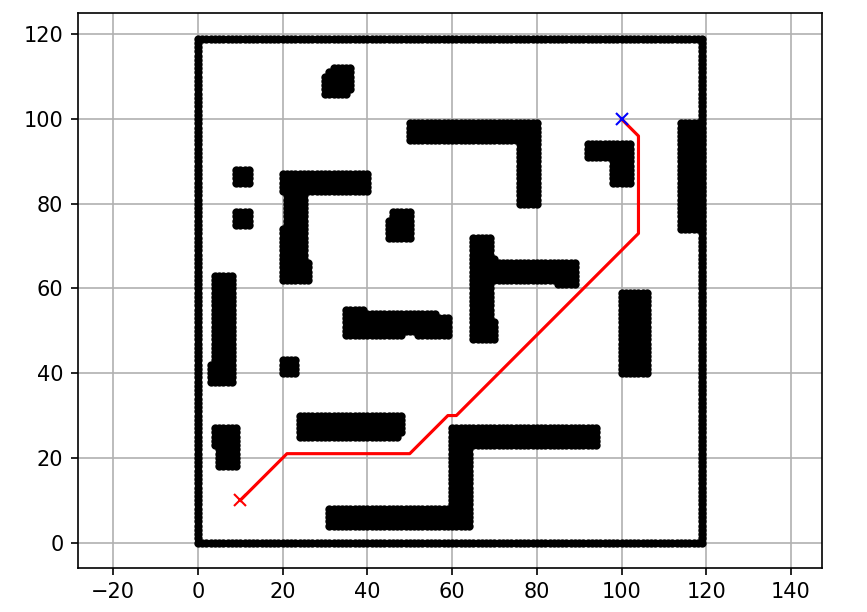
\includegraphics[width=0.4\textwidth]{task2.png} % 插入图片,设置宽度为文本宽度的一半
    \caption{Path for task2} % 设置图片标题
    \label{fig:logo} % 设置标签,用于在文本中引用
\end{figure}
This figure presents the path planned by the improved A$^*$ algorithm from Task 2. The path now includes diagonal movements, allowing for a more direct and shorter route. Besides, it maintains a safer distance from obstacles. Furthermore, the path exhibits fewer unnecessary turns and appears smoother. Overall, the resulting path is qualitatively superior to that of Task 1, showing significant improvements in safety, efficiency, and smoothness.

\newpage
\subsection{Task 3: Path Planning for Self-driving}
\subsubsection{Description}
The objective of Task 3 is to address the  drawback of the paths generated in the previous two tasks: due to the discretization of the map, the paths consist of a series of straight-line segments with sharp turns at corners , which is bad for self-driving vehicles.

To achieve path smoothing, we adopt a two-stage optimization strategy. First, we use a basic A$^*$ algorithm to rapidly obtain an initial and feasible path from the start to the goal. Then we apply an iterative optimization method on the path.  In each iteration, every point on the path is subjected to two competing forces: a "smoothing force" that makes the path more smooth, and an "obstacle repulsion force" that pushes it away from nearby obstacles. After multiple iterations, the path naturally relaxes into an ideal trajectory that is both smooth and safe.

\subsubsection{Formulation}
The algorithm is implemented in two core stages: base path planning and iterative path smoothing.

\paragraph{Stage 1: Basic A$^*$ Path Planning}
The goal of this stage is to quickly obtain a feasible path. We use the same function as Task 1: $f(n) = g(n) + h(n)$, where:
\begin{itemize}
    \item $g(n)$ (Actual Cost): Consider only the movement cost for eight directions (1 for straight, $\sqrt{2}$ for diagonal).
    \item $h(n)$ (Heuristic Function): Employ the Euclidean distance to estimate the cost to the goal.
\end{itemize}
\textit{Note: Here the A$^*$ algorithm in this stage is simplified and does not include the steering and obstacle costs from Task 2, because its purpose is to rapidly obtain a feasible path. We will consider that two costs later in the iterative part.}

\paragraph{Stage 2: Iterative Path Smoothing}
This stage iteratively updates the position of every point $P_i$ on the path, except for the start and end points. In each iteration, the new position $P_i'$ is determined by the vector sum of its current position and two forces:
$$ P_i' = P_i + \vec{F}_{\text{smooth}} + \vec{F}_{\text{obstacle}} $$
\begin{enumerate}
    \item \textbf{Smoothing Force ($\vec{F}_{\text{smooth}}$)}: This force aims to minimize the path's curvature, making it smoother. It pulls the current point towards the midpoint of its two neighbors, formulated as:
    $$ \vec{F}_{\text{smooth}} = \alpha (P_{i-1} + P_{i+1} - 2P_i) $$
    where $\alpha$ is a tunable smoothing weight.
	The following picture is an example of the application of smoothing force on a path with sharp fluctuations.
	\begin{figure}[h!]
		\centering % 图片居中显示
		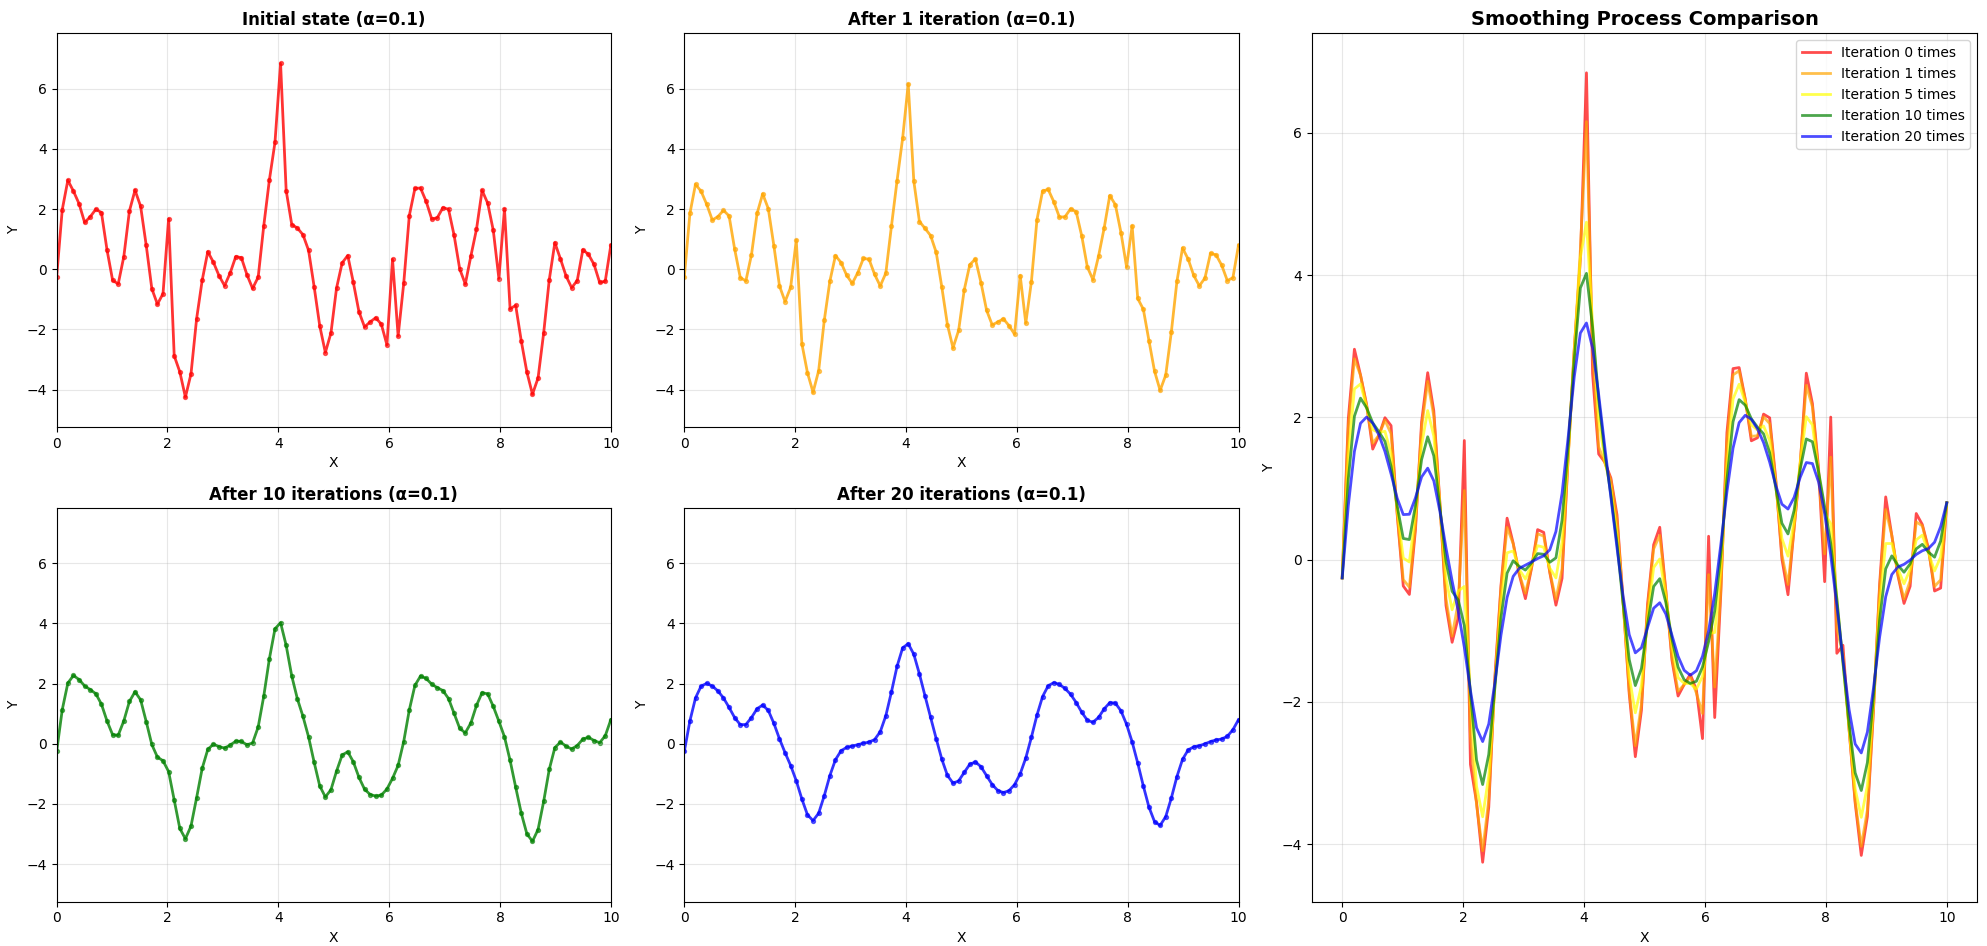
\includegraphics[width=0.9\textwidth]{smooth_force.png} % 插入图片,设置宽度为文本宽度的一半
		\caption{Example for smoothing force($\alpha=0.1$)} % 设置图片标题
		\label{fig:logo} % 设置标签,用于在文本中引用
	\end{figure}


	\newpage
    \item \textbf{Obstacle Repulsion Force ($\vec{F}_{\text{obstacle}}$)}: This force is activated only when a node enters a "danger zone" within a specific distance ($R$) of an obstacle , which means this node is too close to an obstacle. Its direction is determined by the gradient $\nabla D(P)$ of a pre-computed obstacle distance field $D(P)$, always pointing away from the obstacle. It is formulated as :
    $$
    \vec{F}_{\text{obstacle}} = 
    \begin{cases} 
      \beta \frac{R - d(P_i)}{R} \cdot \frac{\nabla D(P_i)}{||\nabla D(P_i)||} & \text{if } d(P_i) < R \\
      0 & \text{if } d(P_i) \ge R
    \end{cases}
    $$
    where $\beta$ is the repulsion weight and $d(P_i)$ is the distance from point $P_i$ to the nearest obstacle.

	\begin{figure}[h!]
		\centering % 图片居中显示
		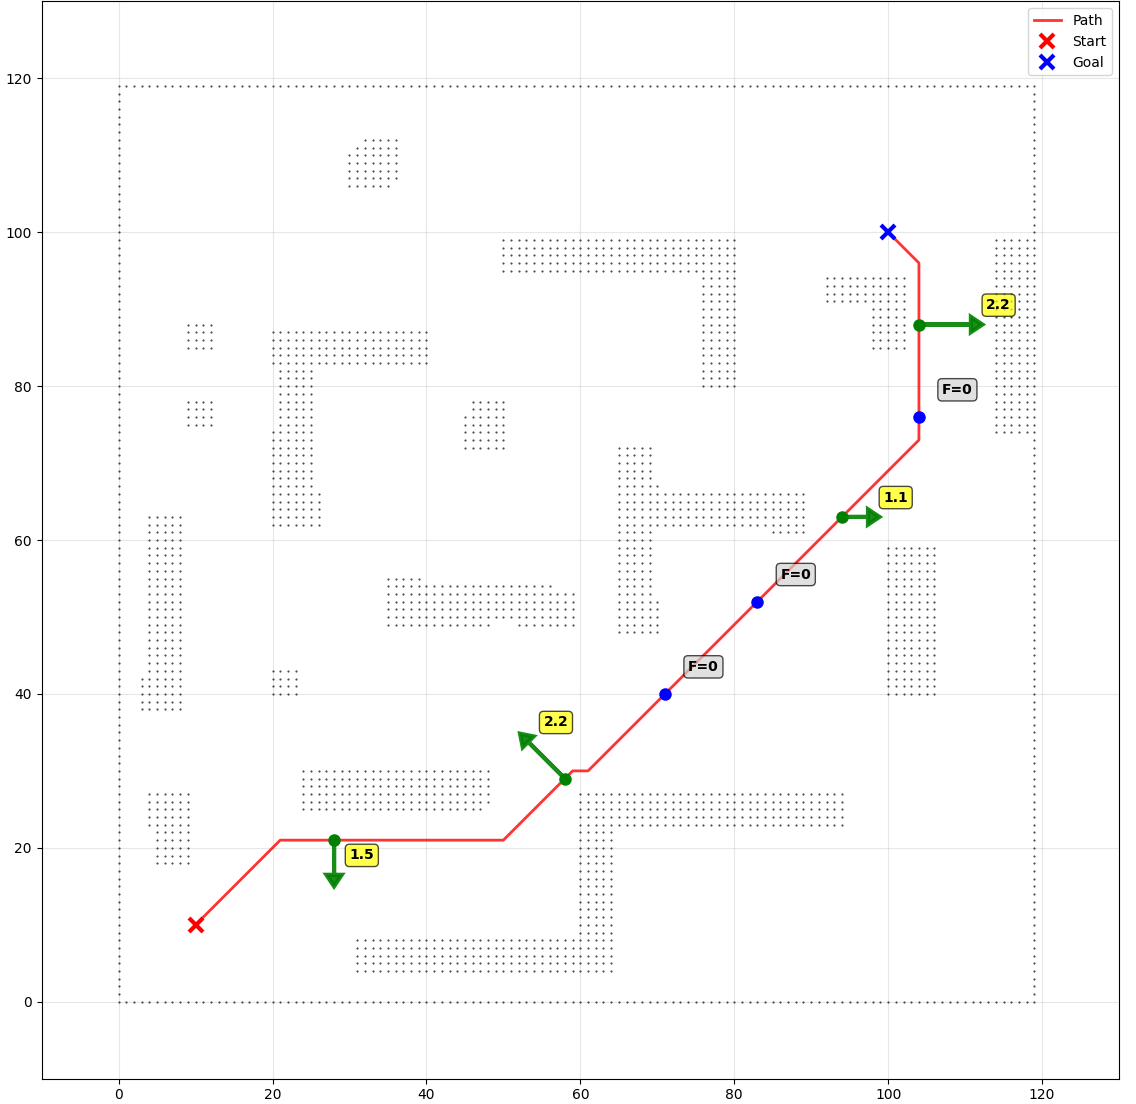
\includegraphics[width=0.4\textwidth]{obstacle_force.png} % 插入图片,设置宽度为文本宽度的一半
		\caption{Example for obstacle repulsion force($\beta = 3 ,R =8$)} % 设置图片标题
		\label{fig:logo} % 设置标签,用于在文本中引用
	\end{figure}
	As shown in the figure , the closer one node is to the obstacle , the bigger its $\vec{F}_{\text{obstacle}}$ is.
\end{enumerate}

\subsubsection{Implementation}
The code's implementation has two stages.

\paragraph{Stage 1: Basic A$^*$ Path Planning}
The code first executes an A$^*$ search. Similar to the previous tasks, it utilizes the Node class, a  min-heap containing nodes, and an explored set. The cost calculation is simplified: the actual cost $g$ accumulates only movement costs, and the heuristic function $h$ uses the Euclidean distance. This stage will quickly outputs a feasible path.

\paragraph{Stage 2: Iterative Path Smoothing}
This is the core of the algorithm, accomplished within a nested loop:
\begin{enumerate}
    \item \textbf{Initialization}: The code first defines some key smoothing parameters: $\alpha$(smoothing weight), $\beta$(repulsion weight), $R$(influence radius), and $iteration$ (the number of iterations).
    
    \item \textbf{Distance Map Pre-computation}: Before the main loop, the \texttt{distance} function is called to generate a \texttt{dist\_map}.
    
    \item \textbf{Main Optimization Loop}: The code iterates over all intermediate points of the path for a total of \texttt{iterations} times.
    
    \item \textbf{Force Calculation}:
    \begin{itemize}
        \item \texttt{smoothing\_force} is directly calculated by \texttt{alpha * (smoothed\_path[i-1] + smoothed\_path[i + 1] - 2 * current\_point)}.
        \item \texttt{obstacle\_force} is calculated if \texttt{dist < influence\_radius}. The gradient direction, \texttt{grad}, is approximated using finite differences (e.g., \texttt{dist\_map[x+1,y] - dist\_map[x-1,y]}). The force magnitude, \texttt{force\_magnitude}, is then calculated based on the distance.
    \end{itemize}
    
    \item \textbf{Collision Detection}: After calculating a candidate \texttt{new\_pos}, the code will check whether it falls within an obstacle cell , which ensures the final smoothed path remains collision-free.
\end{enumerate}

\subsubsection{Parameter Tuning}
After multiple rounds of experimentation and parameter tuning, the current set of values (\texttt{alpha = 0.15}, \texttt{beta = 0.2}, \texttt{influence\_radius = 5.0}, \texttt{iterations = 100}) was determined to be a near-optimal solution for the path smoothing algorithm. 

During the tuning process, I observed that an excessively large \texttt{alpha} value caused the path to shrink, while a value that was too small could cause insufficient smoothing. The \texttt{beta} and \texttt{influence\_radius} parameters both influence the obstacle avoidance effect; higher values led to unnecessarily long paths that stayed far from obstacles, while lower values could lack safety. The \texttt{iteration} parameter directly impacts the algorithm's convergence and computational cost: too few iterations result in an under-smoothed path, while too many lead to unnecessary time consumption. 

The selected parameters achieve an excellent balance between path smoothness, safe distance from obstacles, and overall path length, generating a high-quality path for the given map.

\subsubsection{Result}
\begin{figure}[h!]
	\centering % 图片居中显示
	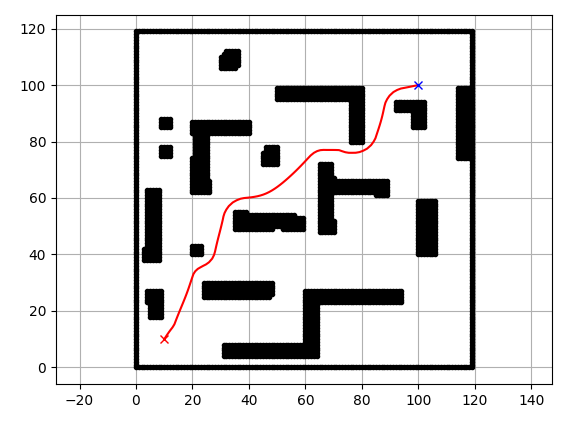
\includegraphics[width=0.4\textwidth]{task3.png} % 插入图片,设置宽度为文本宽度的一半
	\caption{Path for task3} % 设置图片标题
	\label{fig:logo} % 设置标签,用于在文本中引用
\end{figure}
This figure presents the final output of the path smoothing algorithm from Task 3. The algorithm has successfully transformed the discrete, jagged path from the initial A$^*$ search into a continuous and smooth one. While ensuring the path remains entirely collision-free, this method eliminates all sharp turns. %%%%%%%%%%%%%%%%%%%%%%%%%%%
%%%%%%%%%%%%%%%%%%%%%%%%%%%%%%
\newpage
\section{Performance Comparison: Basic A$^*$ vs. Improved A$^*$}

To quantitatively evaluate the performance improvement of the improved A$^*$ algorithm (Task 2) over the basic version (Task 1), we conducted a comparison based on four key metrics: computational time, path length, smoothness (number of turns) and safety (minimum distance to obstacles). 


\begin{table}[h!]
    \centering
    \caption{Comparison of Basic A$^*$ and Improved A$^*$ Algorithms}
    \label{tab:comparison}
    \begin{tabular}{|l|c|c|p{4cm}|}
        \hline
        \textbf{Key Metric} & \textbf{Basic A$^*$ (Task 1)} & \textbf{Improved A$^*$ (Task 2)}  \\
        \hline
        Computational Time (s) & 0.003 s & 0.321 s  \\
        \hline
        Path Length (m) & 180 m & 149 m  \\
        \hline
        Number of Turns & 3 & 6  \\
        \hline
        Min Distance to Obstacle (m) & 1 m &2 m \\
        \hline
    \end{tabular}
\end{table}

\paragraph{Detailed Analysis}
\begin{itemize}
    \item \textbf{Computational Time}: The data shows that the computational time of the improved algorithm (0.321s) is higher than that of the basic version (0.003s). This is expected. The cost function of the basic A$^*$ involves only simple integer additions and Manhattan distance calculations. In contrast, the improved A$^*$ performs more complex operations at each step, including floating-point arithmetic calculations (Euclidean distance), conditional checks (steering cost), and table lookups (obstacle cost), leading to a significant increase in runtime.

    \item \textbf{Path Length \& Optimality}: The improved algorithm excels in path length, reducing the total distance from 180m to 149m. This is attributed to its ability to perform eight-directional movement. By taking diagonal "shortcuts," the path can tend more directly towards the goal.

    \item \textbf{Safety}:The improved algorithm successfully increases the minimum safe distance from 1m to 2m by introducing an \textbf{obstacle avoidance cost}。
    \item \textbf{Number of Turns \& Smoothness}: A counter-intuitive observation is that the number of turns for the improved algorithm (6) is higher than that of the basic version (3), despite the introduction of a \textbf{steering cost}. This is because while the basic path has fewer turns, it is a longer and simpler route. The improved algorithm, has to satisfy the conflicting goals of "taking diagonals" and "staying away from obstacles" in narrow spaces, so it is forced to make more small turns. 
\end{itemize}

%% THIS IS FROM A DIFFERENT CLASS, BUT DEMONSTRATES MATH MODE WELL
%%%%%%%%%%%%%%%%%%%%%%%%%%%%%%
\newpage
\section{Discussion and Conclusion}

\subsection{Discussion of Results}
This assignment successfully implements and progressively optimizes a path-planning system based on the A$^*$ algorithm. Based on the results from the above three tasks, stated below are some key observations:

\begin{enumerate}
    \item \textbf{Effectiveness of the Improved A$^*$ Algorithm}: The comparative results (see Table 1) clearly demonstrate that the improved A$^*$ algorithm from Task 2 is far superior to the basic version from Task 1 in terms of path quality. By enabling eight-directional movement, the path length was significantly reduced from 180m to 149m. At the same time, the introduction of an obstacle avoidance cost successfully increased the minimum safe distance from 1m to 2m, thus enhancing safety. However, this improvement comes at a cost. The more complex cost function led to an increase in computation time from 0.003s to 0.321s, so the designers should balance between path quality and computational efficiency.

    \item \textbf{Necessity of Path Smoothing}: The result of Task 3 demonstrates that path smoothing is not merely an aesthetic enhancement but also a critical step in translating an abstract algorithmic solution into a feasible path in the physical world. The discrete path output by the A$^*$ algorithm cannot be directly executed by a real vehicle for several reasons:
    \begin{itemize}
        \item \textbf{Kinematic Constraints}: Physical vehicles have inertia and are subject to kinematic constraints, such as a minimum turning radius . They cannot perform an instantaneous 90-degree turn. So following a path filled with sharp corners is physically impossible.
        
        \item \textbf{Passenger Comfort}: Every sharp turn produces a sudden lateral acceleration . Such motion makes the passengers feel uncomfortable.   
    \end{itemize}
\end{enumerate}
\subsection{Conclusion}
In conclusion, this assignment successfully constructed and validated a  path-planning algorithm step by step. We began by implementing a basic A$^*$ algorithm, then enhanced it with a composite cost function to significantly improve optimality and safety. Finally, we implemented an smoothing algorithm that successfully transformed the discrete path into a continuous trajectory suitable for real world applications.

Through this project, I have gained a deep understanding that the performance of the A$^*$ algorithm is highly dependent on the design of its cost function, and that path planning often requires making trade-offs between multiple key metrics (e.g., efficiency, safety, length, and smoothness). Also ,  the two-stage optimization method used in Task 3 demonstrates an effective approach to solving complex planning problems: first, use a fast algorithm to solve the core problem (connectivity), and then optimize other performance indicators. This methodology holds high value for me in solving other problems.



%%%%%%%%%%%%%%%%%%%%%%%%%%%%%%
%%%%%%%%%%%%%%%%%%%%%%%%%%%%%%
\newpage
\section{Appendix}
\appendix
\section{Source Code for Task 1}
\label{sec:appendix_task1}

\begin{lstlisting}[language=Python, caption={Source Code for Task 1 (5-Task\_1.py)}, label={lst:task1_code}, basicstyle=\ttfamily\small, numbers=left, frame=tb, breaklines=true]
import sys
import os
import numpy as np
import matplotlib.pyplot as plt
import time
import heapq

MAP_PATH = os.path.join(os.path.dirname(os.path.abspath(__file__)), '3-map/map.npy')


### START CODE HERE ###
# This code block is optional. You can define your utility function and class in this block if necessary.
class Node:
    def __init__(self, parent_node=None, position=None):
        self.parent_node = parent_node
        self.position = position

        self.g = 0
        self.h = 0
        self.total_cost = 0

    def __eq__(self, other):
        return self.position == other.position
    
    def __lt__(self, other):
        #如果总成本相同,则优先选择启发式成本更低的,使其更快到达终点(似乎加了这两行会减少锯齿,使得路径更平滑,但同时也会变慢)
        if self.total_cost == other.total_cost:
            return self.h < other.h
        return self.total_cost < other.total_cost

###  END CODE HERE  ###


def A_star(world_map, start_pos, goal_pos):
    """
    Given map of the world, start position of the robot and the position of the goal, 
    plan a path from start position to the goal using A* algorithm.

    Arguments:
    world_map -- A 120*120 array indicating current map, where 0 indicating traversable and 1 indicating obstacles.
    start_pos -- A 2D vector indicating the current position of the robot.
    goal_pos -- A 2D vector indicating the position of the goal.

    Return:
    path -- A N*2 array representing the planned path by A* algorithm.
    """
    ### START CODE HERE ###
    
    start_point = Node(None, tuple(start_pos))
    goal_point = Node(None, tuple(goal_pos))
    path = []
    
    # 最小堆实现将被探索的节点,以方便拿到最小cost的节点
    nodes = []
    heapq.heappush(nodes, (start_point.total_cost, start_point))
    
    explored = set()
    
    while nodes:
        _, current_point = heapq.heappop(nodes)
        
        if current_point.position in explored:
            continue
        
        if current_point == goal_point:
            final_path = []
            while current_point is not None:
                final_path.append(list(current_point.position))
                current_point = current_point.parent_node
            path = final_path[::-1]
            break


        possible_moves = [(0, 1), (0, -1), (1, 0), (-1, 0)]
        
        for move in possible_moves:
            
            neighbour = (current_point.position[0] + move[0],current_point.position[1] + move[1])

            if neighbour in explored:
                continue

            #检查坐标是否越界
            map_height, map_width = world_map.shape
            if not (0 <= neighbour[0] < map_height and 0 <= neighbour[1] < map_width):
                continue
            
            #检查该位置是否为障碍物
            if world_map[neighbour[0]][neighbour[1]] != 0:
                continue
            
            neighbour_node = Node(current_point, neighbour)
            neighbour_node.g = current_point.g + 1
            neighbour_node.h = (abs(neighbour_node.position[0] - goal_point.position[0]) + abs(neighbour_node.position[1] - goal_point.position[1]))
            neighbour_node.total_cost = neighbour_node.g + neighbour_node.h
            heapq.heappush(nodes, (neighbour_node.total_cost, neighbour_node))

            explored.add(current_point.position)

    if path == []:
        print("Path not found!")
        return []

    ###  END CODE HERE  ###
    return path


if __name__ == '__main__':

    # Get the map of the world representing in a 120*120 array, where 0 indicating traversable and 1 indicating obstacles.
    map = np.load(MAP_PATH)

    # Define goal position of the exploration
    goal_pos = [100, 100]

    # Define start position of the robot.
    start_pos = [10, 10]

    # Plan a path based on map from start position of the robot to the goal.
    path = A_star(map, start_pos, goal_pos)

    # Visualize the map and path.
    obstacles_x, obstacles_y = [], []
    for i in range(120):
        for j in range(120):
            if map[i][j] == 1:
                obstacles_x.append(i)
                obstacles_y.append(j)

    path_x, path_y = [], []
    for path_node in path:
        path_x.append(path_node[0])
        path_y.append(path_node[1])

    plt.plot(path_x, path_y, "-r")
    plt.plot(start_pos[0], start_pos[1], "xr")
    plt.plot(goal_pos[0], goal_pos[1], "xb")
    plt.plot(obstacles_x, obstacles_y, ".k")
    plt.grid(True)
    plt.axis("equal")
    plt.show()
\end{lstlisting}

\newpage
\section{Source Code for Task 2}
\label{sec:appendix_task2}

\begin{lstlisting}[language=Python, caption={Source Code for Task 1 (5-Task\_1.py)}, label={lst:task1_code}, basicstyle=\ttfamily\small, numbers=left, frame=tb, breaklines=true]
import sys
import os
import numpy as np
import matplotlib.pyplot as plt
import time
import heapq
from collections import deque 

MAP_PATH = os.path.join(os.path.dirname(os.path.abspath(__file__)), '3-map/map.npy')


### START CODE HERE ###
# This code block is optional. You can define your utility function and class in this block if necessary.

class Node:
    def __init__(self, parent_node=None, position=None):
        self.parent_node = parent_node
        self.position = position
        self.g = 0  
        self.h = 0     
        self.total_cost = 0       

    def __eq__(self, other):
        return self.position == other.position
    
    def __lt__(self, other):
        if self.total_cost == other.total_cost:
            return self.h < other.h
        return self.total_cost < other.total_cost

#计算地图上每个点离障碍物有多远
def distance(world_map):
    map_height, map_width = world_map.shape

    # 初始化距离图,所有非障碍物点距离为无穷大
    dist_map = np.full(world_map.shape, float('inf'))
    queue = deque()

    for r in range(map_height):
        for c in range(map_width):
            if world_map[r][c] == 1:
                dist_map[r, c] = 0
                queue.append((r, c))

    while queue:
        r, c = queue.popleft()
        for dr in [-1, 0, 1]:
            for dc in [-1, 0, 1]:
                if dr == 0 and dc == 0:
                    continue
                
                nr, nc = r + dr, c + dc

                if 0 <= nr < map_height and 0 <= nc < map_width:
                    if dist_map[nr, nc] > dist_map[r, c] + 1:
                        dist_map[nr, nc] = dist_map[r, c] + 1
                        queue.append((nr, nc))
    return dist_map

###  END CODE HERE  ###


def Improved_A_star(world_map, start_pos, goal_pos):
    """
    Given map of the world, start position of the robot and the position of the goal, 
    plan a path from start position to the goal using A* algorithm.

    Arguments:
    world_map -- A 120*120 array indicating current map, where 0 indicating traversable and 1 indicating obstacles.
    start_pos -- A 2D vector indicating the current position of the robot.
    goal_pos -- A 2D vector indicating the position of the goal.

    Return:
    path -- A N*2 array representing the planned path by A* algorithm.
    """
    ### START CODE HERE ###
    start_point = Node(None, tuple(start_pos))
    goal_point = Node(None, tuple(goal_pos))
    path = []
    nodes, explored = [], set()
    dist_map = distance(world_map)
    
    #两个惩罚权重,避障和转向
    OBSTACLE_WEIGHT = 10.0  
    STEERING_WEIGHT = 0.8   
    heapq.heappush(nodes, (start_point.total_cost, start_point))

    
    while nodes:
        _, current_point = heapq.heappop(nodes)
        
        if current_point.position in explored:
            continue
        explored.add(current_point.position)
        
        if current_point == goal_point:
            final_path = []
            while current_point is not None:
                final_path.append(list(current_point.position))
                current_point = current_point.parent_node
            path = final_path[::-1]
            break

        possible_moves = [(0, 1), (0, -1), (1, 0), (-1, 0), (1, 1), (1, -1), (-1, 1), (-1, -1)]
        
        for move in possible_moves:
            neighbour_pos = (current_point.position[0] + move[0], current_point.position[1] + move[1])

            map_height, map_width = world_map.shape
            if not (0 <= neighbour_pos[0] < map_height and 0 <= neighbour_pos[1] < map_width) or world_map[neighbour_pos[0]][neighbour_pos[1]] != 0 or neighbour_pos in explored:
                continue
            
            neighbour_node = Node(current_point, neighbour_pos)
            
            move_cost = 1.0 if abs(move[0]) + abs(move[1]) == 1 else 1.414
            
            steering_cost = 0
            if current_point.parent_node is not None:
                prev_move = (current_point.position[0] - current_point.parent_node.position[0],
                             current_point.position[1] - current_point.parent_node.position[1])
                if move != prev_move:
                    steering_cost = STEERING_WEIGHT
            
            neighbour_node.g = current_point.g + move_cost + steering_cost

            #和task1不同的移动方式,导致启发函数不同
            dx = abs(neighbour_node.position[0] - goal_point.position[0])
            dy = abs(neighbour_node.position[1] - goal_point.position[1])
            neighbour_node.h = np.sqrt(dx**2 + dy**2)
            
            dist_to_obstacle = dist_map[neighbour_pos[0], neighbour_pos[1]]
            obstacle_cost = 0

            if dist_to_obstacle <= 3 and dist_to_obstacle > 0:
                obstacle_cost = OBSTACLE_WEIGHT / dist_to_obstacle

            neighbour_node.total_cost = (neighbour_node.g + 
                                         neighbour_node.h + 
                                         obstacle_cost)
            
            heapq.heappush(nodes, (neighbour_node.total_cost, neighbour_node))

    if not path:
        print("Path not found!")
        return []

    ###  END CODE HERE  ###
    return path


if __name__ == '__main__':

    # Get the map of the world representing in a 120*120 array, where 0 indicating traversable and 1 indicating obstacles.
    map = np.load(MAP_PATH)

    # Define goal position of the exploration
    goal_pos = [100, 100]

    # Define start position of the robot.
    start_pos = [10, 10]

    # Plan a path based on map from start position of the robot to the goal.
    path = Improved_A_star(map, start_pos, goal_pos)

    # Visualize the map and path.
    obstacles_x, obstacles_y = [], []
    for i in range(120):
        for j in range(120):
            if map[i][j] == 1:
                obstacles_x.append(i)
                obstacles_y.append(j)

    path_x, path_y = [], []
    for path_node in path:
        path_x.append(path_node[0])
        path_y.append(path_node[1])

    plt.plot(path_x, path_y, "-r")
    plt.plot(start_pos[0], start_pos[1], "xr")
    plt.plot(goal_pos[0], goal_pos[1], "xb")
    plt.plot(obstacles_x, obstacles_y, ".k")
    plt.grid(True)
    plt.axis("equal")
    plt.show()
\end{lstlisting}

\newpage
    \section{Source Code for Task 3}
    \label{sec:appendix_task3}
    
    \begin{lstlisting}[language=Python, caption={Source Code for Task 1 (5-Task\_1.py)}, label={lst:task1_code}, basicstyle=\ttfamily\small, numbers=left, frame=tb, breaklines=true]
    import sys
    import os
    import numpy as np
    import matplotlib.pyplot as plt
    import time
    import heapq
    from collections import deque
    
    MAP_PATH = os.path.join(os.path.dirname(os.path.abspath(__file__)), '3-map/map.npy')
    
    
    ### START CODE HERE ###
    # This code block is optional. You can define your utility function and class in this block if necessary.
    class Node:
        def __init__(self, parent_node=None, position=None):
            self.parent_node = parent_node
            self.position = position
            self.g = 0 
            self.h = 0     
            self.total_cost = 0       
    
        def __eq__(self, other):
            return self.position == other.position
        
        def __lt__(self, other):
            if self.total_cost == other.total_cost:
                return self.h < other.h
            return self.total_cost < other.total_cost
    
    #计算地图上每个点离障碍物有多远
    def distance(world_map):
        map_height, map_width = world_map.shape
    
        # 初始化距离图,所有非障碍物点距离为无穷大
        distance_map = np.full(world_map.shape, float('inf'))
        queue = deque()
    
        for r in range(map_height):
            for c in range(map_width):
                if world_map[r][c] == 1:
                    distance_map[r, c] = 0
                    queue.append((r, c))
    
        while queue:
            r, c = queue.popleft()
            for dr in [-1, 0, 1]:
                for dc in [-1, 0, 1]:
                    if dr == 0 and dc == 0:
                        continue
                    
                    nr, nc = r + dr, c + dc
    
                    if 0 <= nr < map_height and 0 <= nc < map_width:
                        if distance_map[nr, nc] > distance_map[r, c] + 1:
                            distance_map[nr, nc] = distance_map[r, c] + 1
                            queue.append((nr, nc))
        return distance_map
    
    ###  END CODE HERE  ###
    
    
    def Self_driving_path_planner(world_map, start_pos, goal_pos):
        """
        Given map of the world, start position of the robot and the position of the goal, 
        plan a path from start position to the goal using A* algorithm.
    
        Arguments:
        world_map -- A 120*120 array indicating current map, where 0 indicating traversable and 1 indicating obstacles.
        start_pos -- A 2D vector indicating the current position of the robot.
        goal_pos -- A 2D vector indicating the position of the goal.
    
        Return:
        path -- A N*2 array representing the planned path by A* algorithm.
        """
    
        ### START CODE HERE ###
        start_point = Node(None, tuple(start_pos))
        goal_point = Node(None, tuple(goal_pos))
        path = []
        nodes, explored = [], set()
        heapq.heappush(nodes, (start_point.total_cost, start_point))
    
        while nodes:
            _, current_point = heapq.heappop(nodes)
    
            if current_point.position in explored: 
                continue
    
            explored.add(current_point.position)
            
            if current_point == goal_point:
                final_path = []
                while current_point is not None:
                    final_path.append(list(current_point.position))
                    current_point = current_point.parent_node
                path = final_path[::-1]
                break
    
            possible_moves = [(0, 1), (0, -1), (1, 0), (-1, 0), (1, 1), (1, -1), (-1, 1), (-1, -1)]
            
            for move in possible_moves:
                neighbor_pos = (current_point.position[0] + move[0], current_point.position[1] + move[1])
                
                map_height, map_width = world_map.shape
                if not (0 <= neighbor_pos[0] < map_height and 0 <= neighbor_pos[1] < map_width) or world_map[int(neighbor_pos[0])][int(neighbor_pos[1])] != 0 or neighbor_pos in explored:
                    continue
                
                neighbor_node = Node(current_point, neighbor_pos)
    
                move_cost = 1.0 if abs(move[0]) + abs(move[1]) == 1 else 1.414
                neighbor_node.g = current_point.g + move_cost
    
                dx = neighbor_node.position[0] - goal_point.position[0]
                dy = neighbor_node.position[1] - goal_point.position[1]
                neighbor_node.h = np.sqrt(dx**2 + dy**2)
    
                neighbor_node.total_cost = neighbor_node.g + neighbor_node.h
    
                heapq.heappush(nodes, (neighbor_node.total_cost, neighbor_node))
    
        if not path:
            print("Path not found by A*!")
            return []
    
        # 参数 (可调节)
        alpha = 0.15  # 平滑权重
        beta = 0.2    # 障碍物排斥权重
        influence_radius = 5.0 # 障碍物排斥力的影响半径
        iterations = 100 # 迭代次数
    
        smoothed_path = np.array(path, dtype=float)
        map_height, map_width = world_map.shape
        dist_map = distance(world_map)
    
        for _ in range(iterations):
            for i in range(1, len(smoothed_path) - 1):
                current_point = smoothed_path[i]
    
                # 计算平滑力
                smoothing_force = alpha * (smoothed_path[i - 1] + smoothed_path[i + 1] - 2 * current_point)
    
                # 计算障碍物排斥力
                obstacle_force = np.zeros(2)
                x, y = int(current_point[0]), int(current_point[1])
                
                if 0 <= x < map_height and 0 <= y < map_width:
                    dist = dist_map[x, y]
                    
                    if dist < influence_radius:
                        # 使用有限差分法近似距离场的梯度
                        if 0 < x < map_height - 1 and 0 < y < map_width - 1:
                            grad_x = dist_map[x + 1, y] - dist_map[x - 1, y]
                            grad_y = dist_map[x, y + 1] - dist_map[x, y - 1]
                            grad = np.array([grad_x, grad_y])
                            
                            grad_norm = np.linalg.norm(grad)
                            if grad_norm > 1e-6:
                                # 力的方向是梯度方向,大小与beta和距离成反比
                                # 离障碍物越近,(influence_radius - dist)越大,力也越大
                                force_magnitude = beta * (influence_radius - dist) / influence_radius
                                obstacle_force = force_magnitude * (grad / grad_norm)
                
                new_pos = current_point + smoothing_force + obstacle_force
                
                # 碰撞检测
                new_x, new_y = int(new_pos[0]), int(new_pos[1])
                if not (0 <= new_x < map_height and 0 <= new_y < map_width and world_map[new_x, new_y] == 1):
                    smoothed_path[i] = new_pos
    
        path = smoothed_path.tolist()
    
        ###  END CODE HERE  ###
        return path
    
    
    if __name__ == '__main__':
    
        # Get the map of the world representing in a 120*120 array, where 0 indicating traversable and 1 indicating obstacles.
        map = np.load(MAP_PATH)
    
        # Define goal position of the exploration
        goal_pos = [100, 100]
    
        # Define start position of the robot.
        start_pos = [10, 10]
    
        # Plan a path based on map from start position of the robot to the goal.
        path = Self_driving_path_planner(map, start_pos, goal_pos)
    
        # Visualize the map and path.
        obstacles_x, obstacles_y = [], []
        for i in range(120):
            for j in range(120):
                if map[i][j] == 1:
                    obstacles_x.append(i)
                    obstacles_y.append(j)
    
        path_x, path_y = [], []
        for path_node in path:
            path_x.append(path_node[0])
            path_y.append(path_node[1])
    
        plt.plot(path_x, path_y, "-r")
        plt.plot(start_pos[0], start_pos[1], "xr")
        plt.plot(goal_pos[0], goal_pos[1], "xb")
        plt.plot(obstacles_x, obstacles_y, ".k")
        plt.grid(True)
        plt.axis("equal")
        plt.show()
    \end{lstlisting}

\end{document} % DONE WITH DOCUMENT!


%%%%%%%%%%
PERSONAL FAVORITE LAB WRITE-UP STRUCTURE
%%%%%%%%%%
\section{Introduction}
	% No Text Here
	\subsection{Purpose}
		% Lab objective
	\subsection{Equipment}
		% Any and all equipment used (specific!)
	\subsection{Procedure}
		% Overview of the procedure taken (not-so-specific!)
\newpage
\section{Schematic Diagrams}
	% Any schematics, screenshots, block
   % diagrams used.  Possibly photos or
	% images could go here as well.
\newpage
\section{Experiment Data}
	% Depending on lab, program code would be
	% included here without the Estimated and
	% Actual Results.
	\subsection{Estimated Results}
		% Calculated. What it should be.
	\subsection{Actual Results}
		% Measured.  What it actually was.
\newpage
\section{Discussion \& Conclusion}
	% 3 Paragraphs:
		% Restate the objective of the lab
		% Discuss personal trials, errors, and difficulties
		% Conclude the lab


%%%%%%%%%%%%%%%%
COMMON COMMANDS:
%%%%%%%%%%%%%%%%
% IMAGES
begin{figure}[H]
   \begin{center}
      \includegraphics[width=0.4\textwidth]{RTL_SCHEM.png}
   \end{center}
\caption{A screenshot of the RTL Schematics produced from the Verilog code.}
\label{RTL}
\end{figure}

% SUBFIGURES IMAGES
\begin{figure}[H]
  \centering
  \subfloat[LED4 Period]{\label{fig:Per4}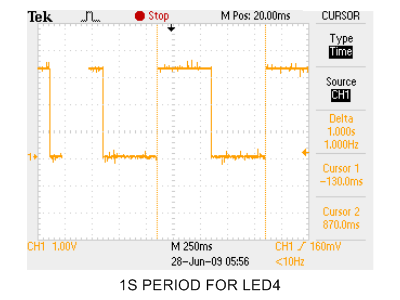
\includegraphics[width=0.4\textwidth]{period_led4.png}} \\
  \subfloat[LED5 Period]{\label{fig:Per5}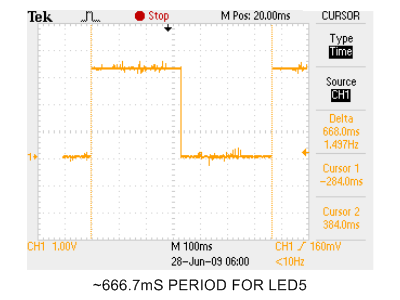
\includegraphics[width=0.4\textwidth]{period_led5.png}}
  \subfloat[LED6 Period]{\label{fig:Per6}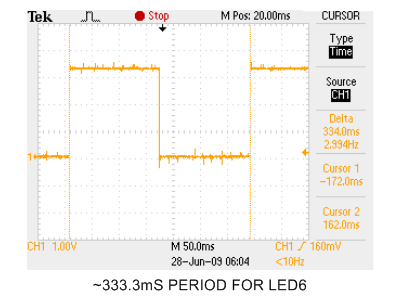
\includegraphics[width=0.4\textwidth]{period_led6.png}}
  \caption{Period of LED blink rate captured by osciliscope.}
  \label{fig:oscil}
\end{figure}

% INSERT SOURCE CODE
\lstset{language=Verilog, tabsize=3, backgroundcolor=\color{mygrey}, basicstyle=\small, commentstyle=\color{BrickRed}}
\lstinputlisting{MODULE.v}

% TEXT TABLE
\begin{table}
\begin{center}
\begin{tabular}{|l|c|c|l|}
	x & x & x & x \\ \hline
	x & x & x & x \\
	x & x & x & x \\ \hline
\end{tabular}
\caption{Caption}
\label{label}
\end{center}
\end{table}

% MATHMATICAL ENVIRONMENT
$ 8 = 2 \times 4 $

% CENTERED FORMULA
\[  \]

% NUMBERED EQUATION
\begin{equation}
	
\end{equation}

% ARRAY OF EQUATIONS (The splat supresses the numbering)
\begin{align*}
	
\end{align*}

% NUMBERED ARRAY OF EQUATIONS
\begin{align}
	
\end{align}

% ACCENTS
\dot{x} % dot
\ddot{x} % double dot
\bar{x} % bar
\tilde{x} % tilde
\vec{x} % vector
\hat{x} % hat
\acute{x} % acute
\grave{x} % grave
\breve{x} % breve
\check{x} % dot (cowboy hat)

% FONTS
\mathrm{text} % roman
\mathsf{text} % sans serif
\mathtt{text} % Typewriter
\mathbb{text} % Blackboard bold
\mathcal{text} % Caligraphy
\mathfrak{text} % Fraktur

\textbf{text} % bold
\textit{text} % italic
\textsl{text} % slanted
\textsc{text} % small caps
\texttt{text} % typewriter
\underline{text} % underline
\emph{text} % emphasized

\begin{tiny}text\end{tiny} % Tiny
\begin{scriptsize}text\end{scriptsize} % Script Size
\begin{footnotesize}text\end{footnotesize} % Footnote Size
\begin{small}text\end{small} % Small
\begin{normalsize}text\end{normalsize} % Normal Size
\begin{large}text\end{large} % Large
\begin{Large}text\end{Large} % Larger
\begin{LARGE}text\end{LARGE} % Very Large
\begin{huge}text\end{huge}   % Huge
\begin{Huge}text\end{Huge}   % Very Huge


% GENERATE TABLE OF CONTENTS AND/OR TABLE OF FIGURES
% These seem to have some issues with the "revtex4" document class.  To use, change
% the very first line of this document to "article" like this:
% \documentclass[aps,letterpaper,10pt]{article}
\tableofcontents
\listoffigures
\listoftables

% INCLUDE A HYPERLINK OR URL
\url{http://www.derekhildreth.com}
\href{http://www.derekhildreth.com}{Derek Hildreth's Website}

% FOR MORE, REFER TO THE "LINUX CHEAT SHEET.PDF" FILE INCLUDED!
